\documentclass[10pt,twocolumn,letterpaper]{article}
\usepackage[pagenumbers]{cvpr}
\usepackage{microtype}
\usepackage[hidelinks]{hyperref}
\graphicspath{{../results/part1-final/}}

\title{Camera Initialization for 3D Gaussian Splatting}
\author{AIAA 3201 Course Project Team}

\begin{document}
\maketitle

\begin{abstract}
We compare COLMAP, VGGT, and VGGT-$\Omega$ as camera and point-cloud initializers for 3D Gaussian Splatting on three course scenes. Each initializer uses the same dense training views for a given scene, and each reconstruction uses a common 7,000-iteration training budget. VGGT-$\Omega$ has the shortest initialization time in all three scenes. The best held-out rendering depends on the scene and metric. Code and aggregate results are available in the \href{https://github.com/MoliaiELS/CV_Project4}{project repository}.
\end{abstract}

\section{Part 1. Pose Initialization for Gaussian Splatting}
\label{sec:part1}

We compare three initializers for novel-view synthesis with 3D Gaussian Splatting (3DGS)~\cite{kerbl2023gaussians}: incremental structure from motion with COLMAP~\cite{schonberger2016sfm}, feed-forward VGGT~\cite{wang2025vggt}, and feed-forward VGGT-$\Omega$~\cite{wang2026vggtomega}. Each initializer estimates camera intrinsics and extrinsics and provides a colored point cloud from the same training images. The downstream optimizer fits the Gaussians while holding the initialized training cameras fixed. We measure both the cost of obtaining an initialization and its effect on pose alignment and held-out rendering after a fixed training budget.

\subsection{Experimental setup}
\label{sec:part1_setup}

\paragraph{Data and split.}
We use the three mandatory scenes, Waymo-405841 and Dl3dv-2 outdoors and Re10k-1 indoors. For each sequence we sort the frame names in natural order and assign every eighth frame, starting with the first, to the test set. Waymo has 174 training and 25 test views, DL3DV has 267 and 39, and RealEstate10K has 244 and 35. The Waymo images are undistorted with the original Brown--Conrady calibration and prepared at $960\times640$ pixels. DL3DV and RealEstate10K images are $256\times256$. All three methods share the same prepared images, training membership, and held-out views for a given scene. The initializers consume training images only.

\paragraph{Camera and point initialization.}
COLMAP 3.11.1 uses CPU SIFT, exhaustive image matching, and incremental mapping with bundle adjustment. We use a shared PINHOLE camera for the Waymo and RealEstate10K video sequences, with intrinsics estimated from the training images, and one PINHOLE camera per image for DL3DV. This configuration registers every training view in all three scenes. The early per-image fits registered 107 of 174 Waymo views and 66 of 244 RealEstate10K views. The reported runs used eight CPU workers on Waymo and RealEstate10K and four on DL3DV. In Waymo we also increased the exhaustive matcher's block size from 50 to 200 after repeated CPU FLANN failures in the multi-block shared-camera run. The larger block covers all 174 training images in one block and keeps the exhaustive image-pair set. The other two scenes use block size 50.

We reuse the official VGGT model code pinned by our earlier VGGT-SLAM project and run it as an offline initializer. VGGT processes the training images jointly at $518\times518$. We offload long-sequence head features to CPU while preserving the joint aggregation across views. VGGT-$\Omega$ uses the official 1B-416 reproduction checkpoint obtained from a verified ModelScope mirror, with balanced preprocessing at $336\times512$ (height by width) for Waymo and $416\times416$ for the two square scenes. Both neural branches predict cameras and depth, map the estimated intrinsics back to the prepared image coordinates, and back-project confidence-filtered depth pixels to colored points without scene-specific bundle adjustment. Each neural run samples 100,000 seed points. The COLMAP point clouds start with 3,112 to 21,831 triangulated points, depending on the scene.

\paragraph{Training and evaluation.}
We use the same gsplat-based 3DGS trainer across methods, with seed 42, 7,000 iterations, and a photometric loss combining L1 and SSIM with an SSIM weight of 0.2. Spherical-harmonic degree rises every 1,000 steps up to degree 3. Densification is enabled from steps 500 to 6,000 at a 100-step interval, with opacity resets every 3,000 steps and a cap of three million Gaussians. We render checkpoints at iterations 500, 1,000, 2,000, 4,000, and 7,000. The completed runs used an RTX 4090, PyTorch 2.6.0 with CUDA 12.4, and gsplat 1.5.3.

We use the course-provided Waymo pose files and the supplied camera tables for DL3DV and RealEstate10K as evaluation references. For each scene and method, we use Umeyama alignment on training camera centers. We fit an estimate-to-reference similarity transformation, Sim(3), and report translation absolute trajectory error (ATE) as the root mean square center residual in reference coordinates. The reference translation units are scene-specific, so we compare ATE within each scene. We fit the reverse direction independently using the same training correspondences, then apply that transform to the held-out reference camera poses. The held-out projections use the reference intrinsics, and rendering uses the resulting cameras without test-view refinement. We average PSNR, SSIM~\cite{wang2004ssim}, and AlexNet LPIPS~\cite{zhang2018lpips} over the held-out views.

Initialization time covers loading, pose and point estimation, and export. The training column gives the time recorded by the optimizer. End-to-end time is the elapsed wall time of the successful run and includes initialization, training, five rounds of rendering and evaluation, and artifact verification. It excludes queue time, environment setup, checkpoint downloads, and previous attempts.

\begin{table*}[t]
  \centering
  \small
  \begin{tabular}{llrrrrrrr}
    \toprule
    Scene & Initializer & PSNR (dB) $\uparrow$ & SSIM $\uparrow$ & LPIPS $\downarrow$ &
    ATE $\downarrow$ & Init. (s) $\downarrow$ & Train (s) & Total (s) $\downarrow$ \\
    \midrule
    Waymo & COLMAP & 17.11 & 0.613 & \textbf{0.440} & \textbf{0.49078} & 805.8 & 186.9 & 1091.2 \\
          & VGGT & \textbf{17.74} & \textbf{0.655} & 0.521 & 0.92756 & 74.7 & 178.1 & 339.4 \\
          & VGGT-$\Omega$ & 16.56 & 0.624 & 0.505 & 0.60770 & \textbf{36.2} & 183.0 & \textbf{308.1} \\
    \midrule
    DL3DV & COLMAP & \textbf{23.61} & \textbf{0.771} & \textbf{0.077} & \textbf{0.01245} & 669.4 & 55.2 & 816.1 \\
          & VGGT & 18.52 & 0.513 & 0.195 & 0.03315 & 122.0 & 72.7 & 250.3 \\
          & VGGT-$\Omega$ & 20.10 & 0.661 & 0.181 & 0.01481 & \textbf{42.1} & 69.9 & \textbf{148.3} \\
    \midrule
    RealEstate10K & COLMAP & 11.07 & 0.276 & 0.392 & 0.01990 & 390.1 & 63.7 & 493.4 \\
                  & VGGT & 11.38 & 0.291 & 0.398 & 0.04512 & 109.6 & 85.0 & 259.6 \\
                  & VGGT-$\Omega$ & \textbf{18.33} & \textbf{0.640} & \textbf{0.068} & \textbf{0.00964} & \textbf{40.2} & 80.7 & \textbf{160.4} \\
    \bottomrule
  \end{tabular}
  \caption{Held-out rendering, aligned training-pose error, and runtime at the 7,000-iteration endpoint. ATE is in each scene's reference translation units. Bold marks the strongest entries within each scene for the direction indicated. Total time includes rendering and evaluation at all five checkpoints.}
  \label{tab:part1_main}
\end{table*}

\subsection{Results}

\paragraph{Quality and runtime at 7,000 iterations.}
Table~\ref{tab:part1_main} shows that the method ranking depends on the scene and metric. In Waymo, VGGT has the highest PSNR and SSIM, while COLMAP has the lowest LPIPS and ATE. In DL3DV, COLMAP leads on all four quality metrics, with a 3.51\,dB PSNR margin over the next best method. On RealEstate10K, VGGT-$\Omega$ has the lowest ATE and the best scores on all three rendering metrics. Its PSNR exceeds VGGT's by 6.95\,dB and COLMAP's by 7.26\,dB. The Waymo result shows that a lower global training camera-center error need not predict the highest held-out pixel agreement in this pipeline.

VGGT-$\Omega$ reduces initialization time relative to VGGT by 2.1--2.9$\times$ and relative to COLMAP by 9.7--22.3$\times$ across the three scenes. It also gives the shortest end-to-end time for each scene, taking 148--308 seconds. Training times are closer within a scene than initialization times. For example, DL3DV's COLMAP run has the shortest training stage at 55.2 seconds, but takes 816.1 seconds end to end, compared with 148.3 seconds for VGGT-$\Omega$. These measurements reflect the study's actual CPU and GPU pipeline configurations.

Optimization ends with 389,467 to 721,872 Gaussians across the nine cases. The smallest final representation is DL3DV with COLMAP, and the largest is RealEstate10K with VGGT. The trainer records 0.66--1.30\,GiB of peak allocated CUDA memory across these runs, measured during 3DGS training.

\begin{figure*}[t]
  \centering
  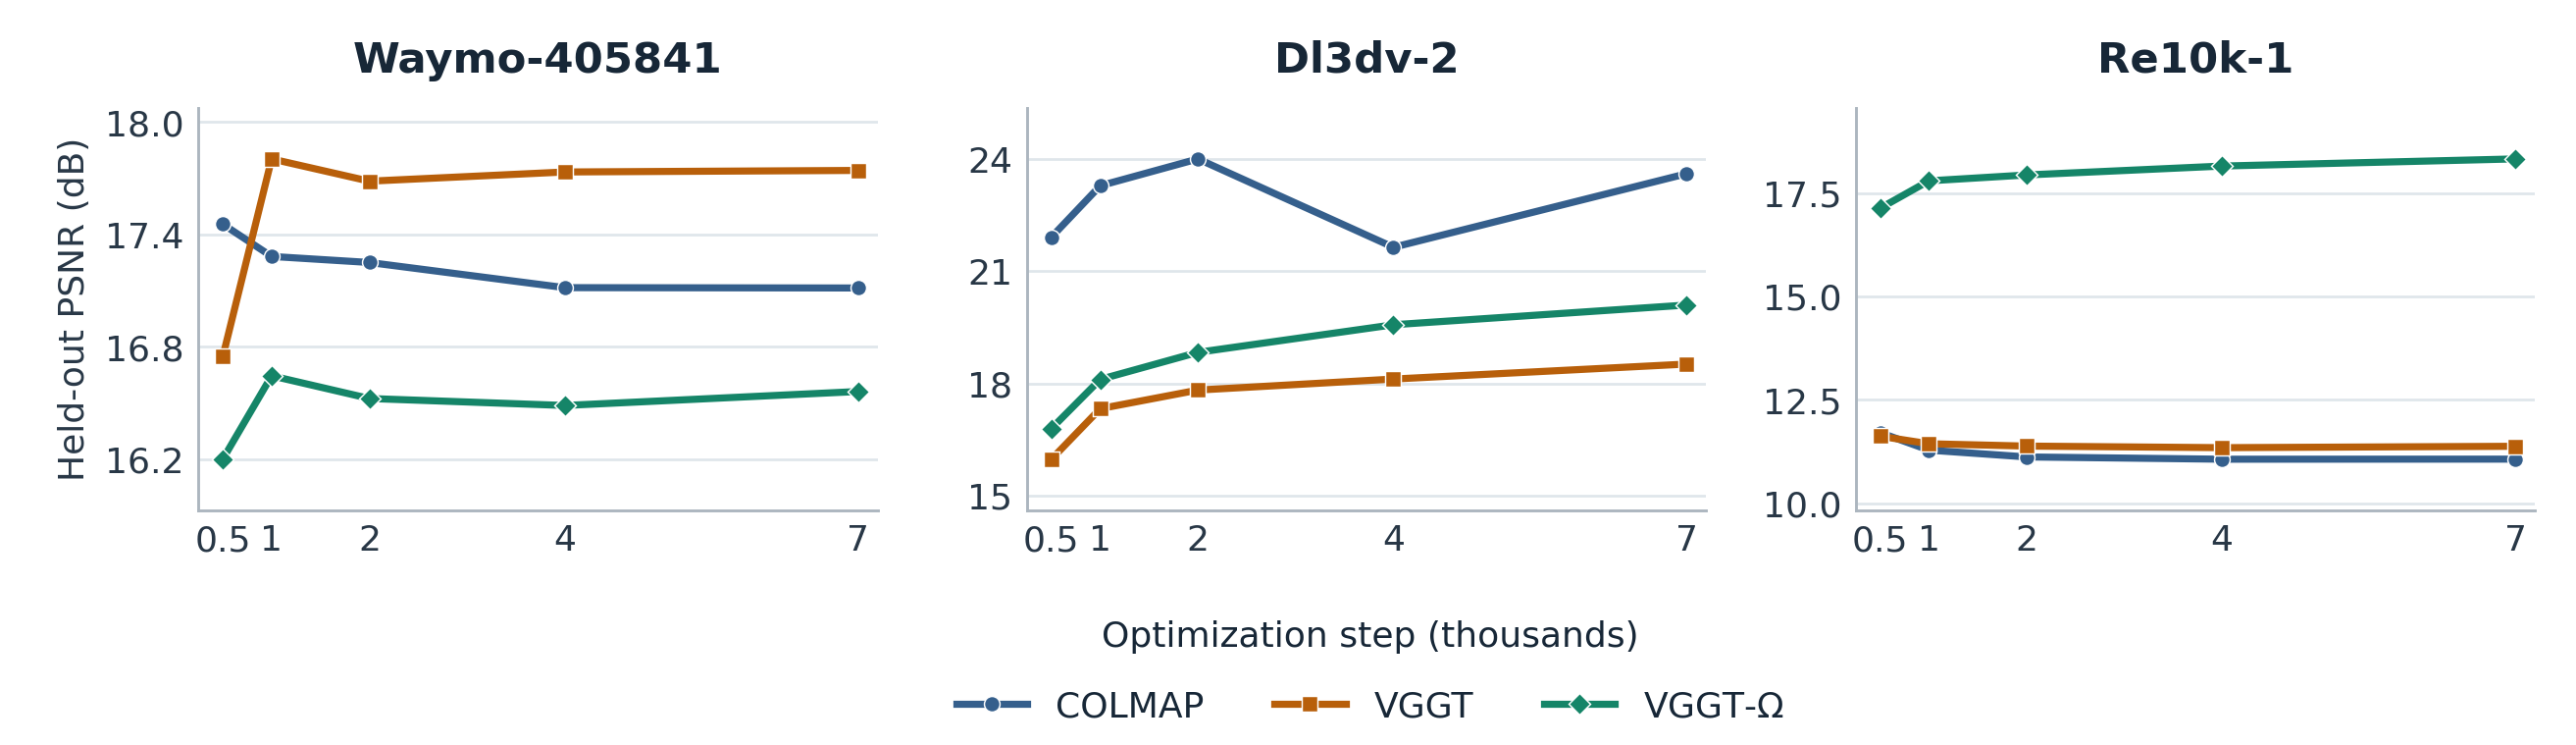
\includegraphics[width=\textwidth]{convergence.png}
  \caption{Held-out rendering at iterations 500, 1,000, 2,000, 4,000, and 7,000. Each point uses the same test views and aligned cameras for its scene and initializer.}
  \label{fig:part1_convergence}
\end{figure*}

\paragraph{Convergence.}
Figure~\ref{fig:part1_convergence} shows that held-out quality can improve or decline under the same iteration schedule. In Waymo, VGGT and VGGT-$\Omega$ reach their highest measured PSNR at 1,000 iterations (17.80 and 16.65\,dB) and finish at 17.74 and 16.56\,dB. COLMAP's PSNR is highest at iteration 500 (17.46\,dB) and declines to 17.11\,dB. In DL3DV, both neural methods improve at every observed checkpoint. COLMAP reaches 24.00\,dB at 2,000 iterations, falls to 21.64\,dB at 4,000, and recovers to 23.61\,dB at 7,000. In RealEstate10K, VGGT-$\Omega$ gains 1.19\,dB between iterations 500 and 7,000, while the COLMAP and VGGT runs peak at the first observed checkpoint. We report the common 7,000-iteration endpoint for all methods.

\IfFileExists{figures/part1_comparison.png}{%
  \begin{figure*}[t]
    \centering
    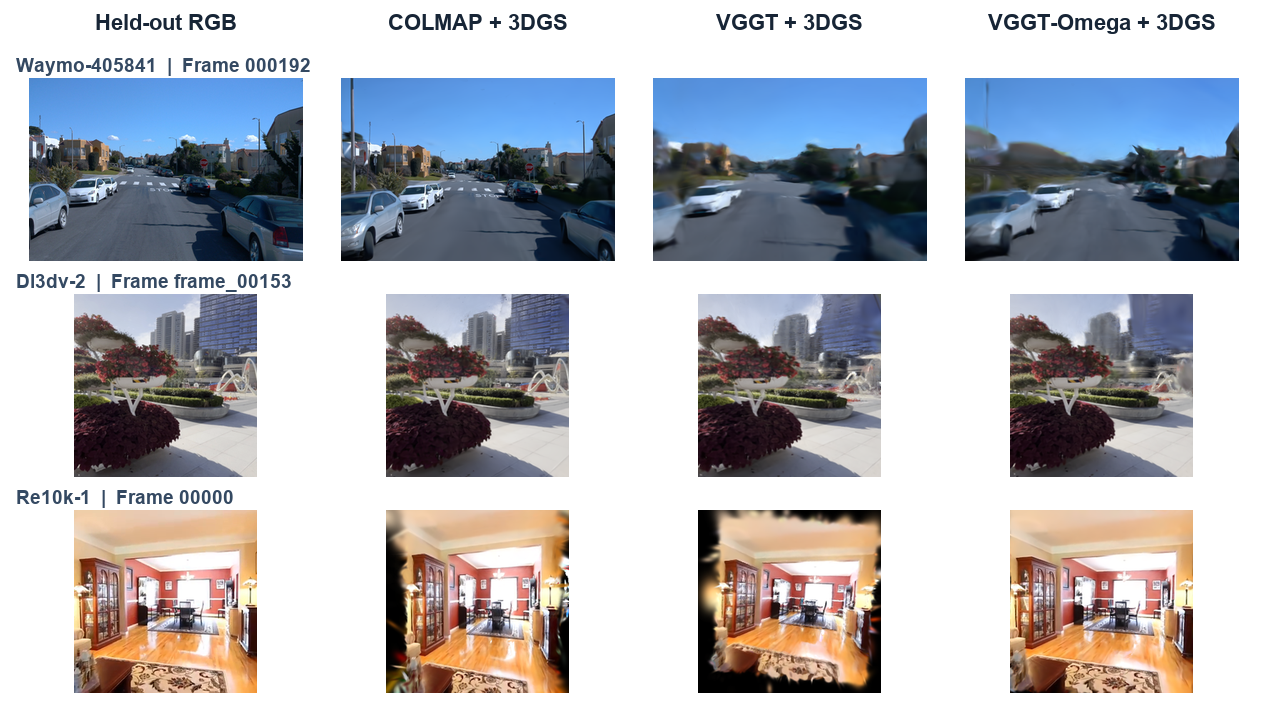
\includegraphics[width=\textwidth]{figures/part1_comparison.png}
    \caption{Representative held-out reference frames and corresponding 7,000-iteration renders from the three initializers.}
    \label{fig:part1_comparison}
  \end{figure*}
}{}

\paragraph{Qualitative comparison.}
\IfFileExists{figures/part1_comparison.png}{Figure~\ref{fig:part1_comparison} shows the renders alongside their reference frames. }{}%
In some held-out Waymo views COLMAP retains sharper road markings and cars. VGGT-$\Omega$ softens parts of the road and its boundary in the first view. In DL3DV, the COLMAP render better preserves foreground contours and the fa\c{c}ade. The learned-initialization renders show visible distortion in background details, including the region above the flower pots in frame 00153. For RealEstate10K, VGGT-$\Omega$ better preserves furniture contours and the image borders, with fewer conspicuous dark bands and edge artifacts than the other initializers in frames 00000 and 00272. These observations describe individual views and complement the scene averages.

\paragraph{Scope and reproducibility.}
This study covers one scene per dataset and one optimization seed. The results depend on the observed scenes, fixed-pose training, preprocessing, and the specific pretrained models and memory settings used here. ATE measures aligned translation alone, while rendering quality also depends on intrinsics, rotation, appearance, and scene coverage. We compare the working initializers as configured and report their complete runtime, with no controlled ablation over neural resolution or over COLMAP's camera-sharing and worker settings. The experiment code underlying the recorded runs is revision \texttt{bde9244f69}. The archived handoff provides per-case metrics at all five checkpoints and a \texttt{checkpoint.json} manifest for each 7,000-iteration model with its server location and checksum.

\bibliographystyle{ieeenat_fullname}
\bibliography{part1_refs}
\end{document}
